
%% this section contains XX problems


%% 2004-APB
%%------------------------------
\element{AP}{
\begin{question}{2004-APB-Q68}
    A constant force of \SI{900}{\newton} pushes a \SI{100}{\kilo\gram}
        mass up the inclined plane shown below at a uniform speed
        of \SI{4}{\meter\per\second}.
    \begin{center}
        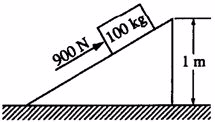
\includegraphics[keepaspectratio]{2004-APB-Q68}
    \end{center}
    The power developed by the \SI{900}{\newton} force is most nearly
    \begin{choices}
        \wrongchoice{\SI{400}{\watt}}
        \wrongchoice{\SI{800}{\watt}}
        \wrongchoice{\SI{900}{\watt}}
        \wrongchoice{\SI{1000}{\watt}}
      \correctchoice{\SI{3600}{\watt}}
    \end{choices}
\end{question}
}

